\chapter{Suunnittelu}
\label{ch:suunnittelu}
Tässä osuudessa käydään toteutetun ohjelman suunnittelu läpi ja kerrotaan miten ja miksi ratkaisuihin päädyttiin. Kappaleissa vertaillaan eri vaihtoehtoja ja peilataan demoversion ongelmia ja niiden perusteella yritetään löytää toimiva ratkaisu ongelmaan. Ensin suunnitellusta ohjelmasta annetaan kattava kokonaiskuva lukijalle ja tämän jälkeen tulevissa kappaleissa mennään jokaisen kohdan yksityiskohtiin tarkemmin.


\section{Kokonaiskuva}
Aikaisemmin kappaleessa \ref{ch:demoversio-ja-sen-toiminta} kuvassa \ref{fig:demo-architecture} esiteltiin demoversion arkkitehtuuri ja sen toiminta. Kuinka viestit IED-laitteelta kulkee ohjelman läpi ja tallennetaan tietokantaan. Tietokannasta muut ohjelmat lukevat tietoa kyselemällä sitä erikseen. Suunnittelun jälkeen demoversion järjestelmästä päädyttiin kuvassa \ref{fig:planned-system-architecture} olevaan järjestelmän arkkitehtuuriin. Kuvassa katkoviivalla on merkitty tässä kappaleessa suunniteltu ohjelmisto. Ja kuvan yläreunassa oleva viiva kuvaa viestin kulkua järjestelmän eri osapuolten läpi ja missä muodossa viesti on missäkin kohtaa.

\begin{figure}[ht!]
	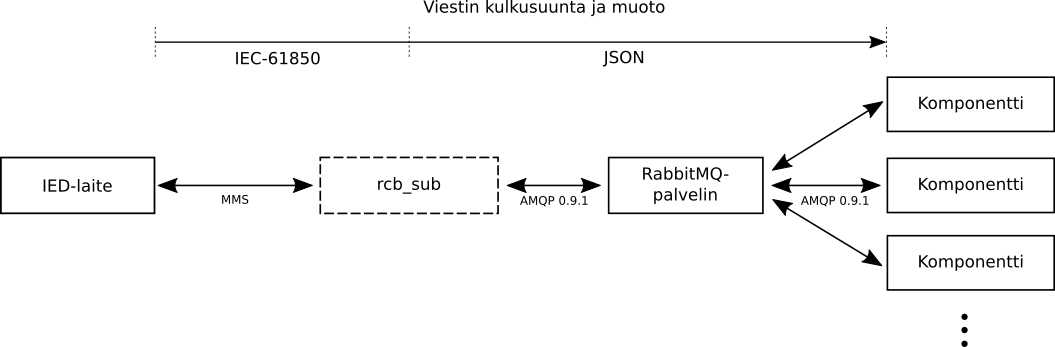
\includegraphics[width=1\textwidth]{pictures/planned-system-architecture.png}
	\caption{Suunnitellun järjestelmän toiminta ja viestin kulkeminen ja muoto eri osapuolten välillä.}
	\label{fig:planned-system-architecture}
\end{figure}

Suunnitellussa arkkitehtuurissa C-kielellä toteutettu ohjelma on komentorivipohjainen ja ei käyttänyt tietokantaa. Kaikki ohjelman ajoon annettavat parametrit annetaan komentoriviparametreille ennen ohjelman käynnistämistä. Demoversio luki tiedot tietokannasta. C-ohjelma voi tilata yhdellä IED-laitteella olevia RCB-instansseja. Tilattuaan RCB-instanssit, ohjelma odottaa viestejä IED-laitteelta IEC 61850 -standardin määrittämässä muodossa. Kun viesti saapuu, ohjelma prosessoi sen ja julkaisee AMPQ-standardin pohjaiselle jonopalvelimelle JSON-muodossa (engl. JavaScrip Object Notation). Lopullisessa toteutuksessa jonopalvelimena käytettiin RabbitMQ-nimistä ohjelmistoa, joka pohjautuu AMPQ-standrdin versioon 0.9.1. Jonopalvelimelta muut tilaavat ohjelmat voivat tilata viestejä, ja viestin saapuessa palvelin ilmoittaa siitä asiakkaalle. Toteutettu C-ohjelmisto käytti edelleen demoversiosta tuttua libiec61850-kirjastoa hoitamaan matalan tason IEC 61850 -standardin määrittämän funktionaalisuuden.


\section{Järjestelmän hajautus ja arkkitehtuuri}
\label{ch:järjestelmän-hajautus-ja-arkkitehtuuri}
Järjestelmän hajauttaminen oli vaatimus uudelle arkkitehtuurille, joka täytyisi ottaa huomioon. Hajautuksella tarkoitetaan että viesteistä kiinnostuneet ohjelmat, pystyisivät niitä tilaamaan ja ottamaan vastaan helposti. Ongelmia ei saisi tulla jos asiakasohjelmia olisi tulevaisuudessa enemmänkin. Demossa erilliset ohjelmat joutuivat lukemaan viestejä jatkuvasti tietokannasta, ilman tietoa siitä milloin uusi viesti olisi saapunut. Tällainen ratkaisu ei tulisi toimimaan pitemmän päälle ja tilanne olisi pahentunut jos tietoa tarvitsevia ohjelmia olisi enemmänkin tulevaisuudessa. Lisäksi tässä toteutuksessa tietokanta on jatkuvan turhan lukemisen ja kuormituksen kohteena. Tilanteeseen tarvittaisiin ratkaisu, jossa tilaava ohjelma voisi tilata viestin ja saada ilmoituksen kun tieto on saatavilla (tilaaja-julkaisija -arkkitehtuuri).

Ratkaisuna olisi voinut ajatella että tietoa tarvitsevat ohjelmat, olisi voineet suoraan tilata viestit IED-laitteelta. Näin kaikki ohjelmat saisivat saman viestin. Kuitenkin tässä esteenä on, että IEC 61850 -standardin määrityksen mukaan yksi RCB-instanssi voi olla vain tilattuna yhdellä asiakkaalle kerrallaan, niinkuin teorian kappaleessa \ref{ch:viestien-tilaus-ja-tilauksen-konfigurointi} käsiteltiin. Ja IED-laitteiden RCB-instanssit ovat rajalliset ja päätetty laitteen konfiguroinnin yhteydessä. Lisäksi IED-laitteet pystyvät rajoittamaan päällä olevien yhteyksien määrää johonkin lukuun. Tavoitteena siis olisi minimoida avoimet yhteydet IED-laitteelle, ja samalla tarjota sama viesti mahdollisimman monelle siitä kiinnostuneelle ohjelmalle. Näistä vaatimuksista päästään ratkaisuun, missä yksi ohjelma tilaa kaikki halutut RCB-instanssit yhdeltä IED-laitteelta. Odottaa viestejä ja lähettää ne edelleen muille niitä tarvitseville ohjelmille. Viestejä tarvitsevien ohjelmien määrä voi vaihdella tarpeen mukaan. Tästä päästään vaatimukseen, että IED-laitteelta viestejä tilaavan ohjelmiston ei tarvitsisi tietää muista tilaavista ohjelmista mitään. Ohjelman pitäisi pystyisi julkaisemaan viestit eteenpäin, välittämättä siitä kuka viestejä vastaanottaa.

Ratkaisuna yllä mainittuihin vaatimuksiin oli sijoittaa IED-laitteen ja muiden tilaavien ohjelmien väliin väliohjelmisto, kuten kuvassa \ref{fig:planned-system-architecture} on C-ohjelma sijoitettu. Näin pystyttiin minimoimaan yhteyksien määrä IED-laitteelle yhteen. Lisäksi sijoittamalla C-ohjelman ja muiden tilaavien ohjelmien väliin jonopalvelin, saadaan aikaan joustavuus mitä haluttiin. C-ohjelman ei tarvitse välittää siitä kuka viestejä vastaanottaa ja jonopalvelimen avulla yhden julkaisijan voi tilata monta erillistä tilaaja. Jonopalvelimen avulla jokainen tilaaja saa saman alkuperäisen viestin, mutta kopiona. Koska standardi ei määrittänyt muita viestien tilaamisen mahdollisuuksia, tämä suunnitelma arkkitehtuurista täytti kaikki sille asetetut vaatimukset.

Demoversiossa ohjelma luki IED-laitteen tiedot kuten IP-osoitteen ja RCB-instanssien referenssit tietokannasta ja tallensi saapuneet viestit tietokantaan. Nyt kun viestit julkaistiin erilliselle jonopalvelimelle, niin tietokantaa ei siihen enää tarvinnut. C-ohjelman tarkoitus oli vain olla väliohjelma viestien välittämiseen eteenpäin, joten siihen ei tarvittu käyttöliitymää. Ohjelmasta päätettiin tehdä komentorivipohjainen toteutus, jolle kaikki tiedot voitaisiin syöttää komentorivillä parametereillä käynnistyksen yhteydessä. Tällä suunnitelmalla toteutus ei tarvitsisi tietokantaa, joten se voitiin jättää pois suunnitelmasta.


\section{Suorituskyky ja kielen valinta}
Demoversio oli ohjelmoitu Ruby-kielellä ja siinä oli paikoin suoritukseen liittyviä ongelmia ja epävarmuutta, etenkin viestien ja RCB-instassien määrän ollessa suurempi. Syitä ja ongelmia käytiin läpi kappaleessa \ref{ch:ongelmakohdat-ja-analysointi}. Oli selvää että ohjelman suorituskykyä täytyi saada parannettua ja siinä olevat ongelmat korjattua (esimerkiksi muistivuoto). Ennen koko ohjelman uudelleenkirjoitusta, Ruby-ohjelmaa kokeiltiin saada toimimaan JRuby\footnote{\url{http://jruby.org/}} nimisellä Ruby-tulkilla. Tavoitteena saada demoversion toteutus toimimaan ilman GIL:iä ja säikeet suoritukseen rinnakkain. JRuby on Ruby-koodin tulkki, joka suorittaa Ruby-lähdekoodia Java virtuaalikoneen (engl. Java Virtual Machine, lyhennetään JVM) päällä. JRuby mahdollistaa säikeiden suorituksen rinnakkain JVM:n omilla säikeillä ja näin ollen suorituksen pitäisi olla nopeampaa \mbox{\cite{Youssef2013}}. Jos tämä lähtökohta olisi toiminut, olisi edelleen järjestelmän arkkitehtuuria pitänyt muuttaa samaan suuntaan, kuin kappaleessa \ref{ch:järjestelmän-hajautus-ja-arkkitehtuuri} kuvattiin. Tämän lisäksi demossa oleva muistivuoto olisi pitänyt korjata. JRuby ei kuitenkaan toiminut ja nopean yrityksen jälkeen päätettiin vain palata suunnitelmaan kirjoittaa koko ohjelma uudestaan. Syynä tähän oli että demoversio oltiin tehty osaksi isompaa Rails projektia, joka toimi Rubyn oletustulkin päällä. Ja JRuby ei tukenut kaikkia projektin kirjastoja mitä se käytti. Rubyssä kirjastoja kutsutaan jalokiviksi (engl. gem). Seurauksena olisi ollut saman projektin ylläpitäminen kahdelle eri tulkille tai asennettavien pakettien erottaminen. Kuitenkaan yrittämisen jälkeen tätäkään ei saatu toimimaan. Lisäksi täytyi ottaa huomioon implementaatioon käytetty aika ja useat mahdolliset viat jotka olisi täytynyt korjata.

Kysymksenä tämän aikana tuli ajan käyttö ja fakta että demosta olisi pitänyt korjata ja paikata monta asiaa. Päätyttiin toteuttamaan koko ohjelmisto uudestaan kielellä jossa ei olisi suorituskykyongelmia. Samalla uudessa toteutuksessa ohjelma voitiin toteuttaa tekemään asetetut tavoitteet ja demoversion ongelmia ei tarvitsisi korjata.

Uuden toteutuksen kieleksi valittiin C-kieli. Isona syynä kielen valintaan oli tekijän iso mieltymys matalan tason ohjelmointiin ja C-kieleen. Lisäksi C-kieli käännetään alustalle suoraan konekäskyiksi, joiden suoritus on nopeampaa kuin tulkattavan kielen, kuten Ruby ja Python. Kielen valinnan yhteydessä kuitenkin oli hyvä varmistaa kaikkien suunniteltujen liitosten mahdollisuus. C-kielelle löytyi kirjastoja RabbitMQ-jonopalvelimen käyttämiseen ja lisäksi JSON rakenteen muodostamiseen. Hyötynä vielä C-kielen valinnasta oli, että demossa käytettyä libIEC61850 kirjastoa pystyi käyttämään suoraan ilman erillistä liitosta, koska kirjasto oli myös tehty C-kielellä. Tarkemmin käytettyihin kirjastoihin ja toteutukseen pureudutaan kappaleessa \ref{ch:toteutus}.


\section{Prosessoidun viestin muoto ja rakenne}
Saapuva viesti esitettiin libIEC61850-kirjastossa ClientReport struktuurin instanssina. Stuktuuri sisältää viestin datan ja sen voi lukea käyttämällä kirjaston tarjoamia funktioita \mbox{\cite{libIEC61850-doc}}. Saapunut viesti haluttiin jakaa jonopalvelimen läpi muille osapuolille, joten viestin täytyi olla helposti luettavassa muodossa muille ohjelmille. Viesti päädyttiin muuttamaan helposti ymmärrettäväksi JSON-rakenteeksi. JSON-rakenteen voi helposti ihminen lukea ja se on nykypäivänä paljon käytetty tiedonsiirtomuoto erilaisissa web-palveluissa ja rajapinnoissa. Myöskin JSON-rakenteiden lukemiseen on monelle eri kielellä olemassa valmiita kirjastoja sen monikäyttöisyyden takia \mbox{\cite{Patrizio2016}}.

Liitteessä \ref{ch:report-json-format} on esitetty prosessoidun JSON-rakenteen muoto johon tässä työssä päädyttiin ja toteutettu C-ohjelma lopulta julkaisi RabbitMQ-jonopalvelimelle. Standardin määrittämää viestin rakennetta ja sisältöä käytiin läpi kappaleessa \ref{ch:viestin-rakenne}. JSON:in rakenne noudattaa pääasissa standardin määrittämää viestin rakennetta, mutta joitakin asioita on tehty toisin. Lisäksi C-ohjelma myös lisäsi viestiin lisää tietoa attribuuteista selkeyden takia (kuten viitteen, tyypin ja koon). Kuinka tämä toteutettiin käsitellään tarkemmin kappaleessa \ref{ch:toteutus}.

Standardin viestin kenttien määrää pystyi säätämään RCB-instanssin OptFlds-attribuutilla. JSON:iin kuitenkin haluttiin lisätä kaikki mahdolliset kentät selkeyden vuoksi. Joten jos kenttä viestistä puuttui, asetettiin sen arvoksi JSON:issa null. Esimerkiksi liitteessä \ref{ch:report-json-format} kentän confRevision arvo on null. Eli tällöin RCB-instanssissa OptFlds-attribuutin conf-revision on ollut epätosi. Sama käytäntö toistettiin kaikille muillekin vaihtoehtoisille kentille. Tällä periaatteella viestin OptFlds-kenttä voitiin jättää pois JSON:ista. JSON:iin päädyttin lisäämään FCD- ja FCDA-viitteiden alla viitatut oikeat attribuutien viitteet, tyyppit ja koot arvojen lisäksi. Tämä toteutettiin selkeyden takia ja näin voidaan päätellä mitkä arvot oikeasti kuuluvat viestiin ja mitkä ovat niiden viitteet. Standardissa viesti sisälsi vain datajoukon FCD- tai FCDA-viitteen ja taulukon arvoja mihin sen alla viitattiin. Liitteessä \ref{ch:report-json-format} oleva JSON-rakenne koostuu kahdesta sisäkkäisestä values-attribuutista (rivit 7 ja 13). Rivillä 7 oleva values-taulukko sisältää viestissä olevat datajoukon FCD- tai FCDA-viitteet ja niihin liittyvät kentät. Samalla periaattelle kuin standardin määrittämässä viestin rakenteessa kuvassa \ref{fig:iec61850-report-format} olevat taulukon arvot 1--n:ään. Eli viestin Reason Code on laitettu reasonForInclusion attribuuttiin. Viestin DataRef-kenttä on pilkottu kolmeen eri kenttään mmsReference, reference ja functionalConstraint. Viestien viitteet tulevat MMS-protokollamäärityksen muodossa eli pisteet (.) on korvattu dollarilla (\$) ja viite sisältää funktionaalisen rajoitteen. Nyt mmsReference sisältää viestin alkuperäisen MMS-viitteen, reference sisältää standardin abstraktin viitteen ja functionalConstraint sisältää funktionaalisen rajoitteen. Nämä on erotettu selkeyden takia, koska mahdollisesti jotkin asiakasohjelmat saattavat tarvita standardin käyttämää abstraktia viitettä. Näin asiakasohjelma välttää teksimuunnokset. JSON:in sisempi values-attribuutti (liitteessä \ref{ch:report-json-format} ensimmäinen rivillä 13) sisältää taulukon itse viestin arvoista. C-ohjelma lisää niihin oikeat viitteet, tyypin ja koon. Poikkeuksena boolean ja utc-time tyypit, jolla ei ole kokoa ollenkaan. Koko kertoo monellako bitillä kyseinen attribuutti esitetään ja se voi vaihdella saman tyypin välillä (esimerkiksi bit-string). Myöskin bit-string tyypille päädyttiin lisäämään kaksi eri arvoa valueLittleEndian ja valueBigEndian. Tämä sen takia, koska tavujärjestys ei ole vältämättä tiedossa missä järjestyksessä bitit muuttujassa ovat päätettiin tarjota kummatkin vaihtoehdot asiakkaalle. Ajat päätettiin antaa suoraan siinä formaatissa, missä ne tulevat viestissä. Eli viestin päätason aikaleima on millisekunteja UNIX-ajanlaskun alusta 1. tammikuuta 1970 klo 00:00:00 UTC tähän hetkeen. Attribuuteissa tyypiltään utc-time, luku on sekunteja samasta UNIX-ajanlaskusta tähän hetkeen \mbox{\cite[s.~26--27]{IEC61850-7-2}}.